\chapter{Introduction}~\label{chp:INTRO}

The QWeak simulation package {\em QweakSimG4} is a collection of C++
{\em classes} that can be compiled and run for the purpose of physics
process simulation in the experiment. The code aims to eventually
include all objects and properties found in the current design of the
QWeak experiment, as well as most physics processes that are expected
to emerge during the experiment. The implementation of these objects
and properties is at various stages of development, the detail of
which is indicated in the extent of the list of contents.  The code is
based on the GEANT4\footnote{{\tt
http://wwwasd.web.cern.ch/wwwasd/geant4/geant4.html}} simulation
code~\cite{pp:GEANT4} and the ROOT\footnote{ Copyright \copyright
1995-2004 Rene Brun \& Fons Rademakers. All rights reserved.  {\tt
http://root.cern.ch}} analysis package and requires these to compile.

The purpose of this manual is to describe the classes and their
routines and how they are used in the simulation. The manual is
supposed to enable other people to extend, repair or otherwise change
the QWeak simulation program to suit their purposes. Most importantly,
it is meant to document the algorithms used in implementing the
physical processes in the simulation, in as far as they go beyond what
is implemented in GEANT4 itself and adequately described in its
manual. The detail with which the code is described will be evolving
over time. Please make sure that you consult the most recent version
before contacting us with questions. If you cannot find the answer to
your problem in here, you can contact us at {\tt grimm@jlab.org or
mgericke@jlab.org}.

A few points to consider before using this manual are that, (1) we do
not (can not) spent much time explaining any details regarding the
usage of the ROOT or GEANT4 packages and its class libraries. So you
should be or become acquainted with (most) aspects of the packages
before trying to make any serious changes. You can find details about
ROOT and GEANT4 from their websites and the ROOT manual
itself~\cite{tn:ROOT}.  Also, (2) this library is intended to work for
{\em Linux} only. We have made no attempt to make this run on Windows
or Mac.

\clearpage

\begin{landscape}
\begin{figure}[h]
  \hspace{0cm}
  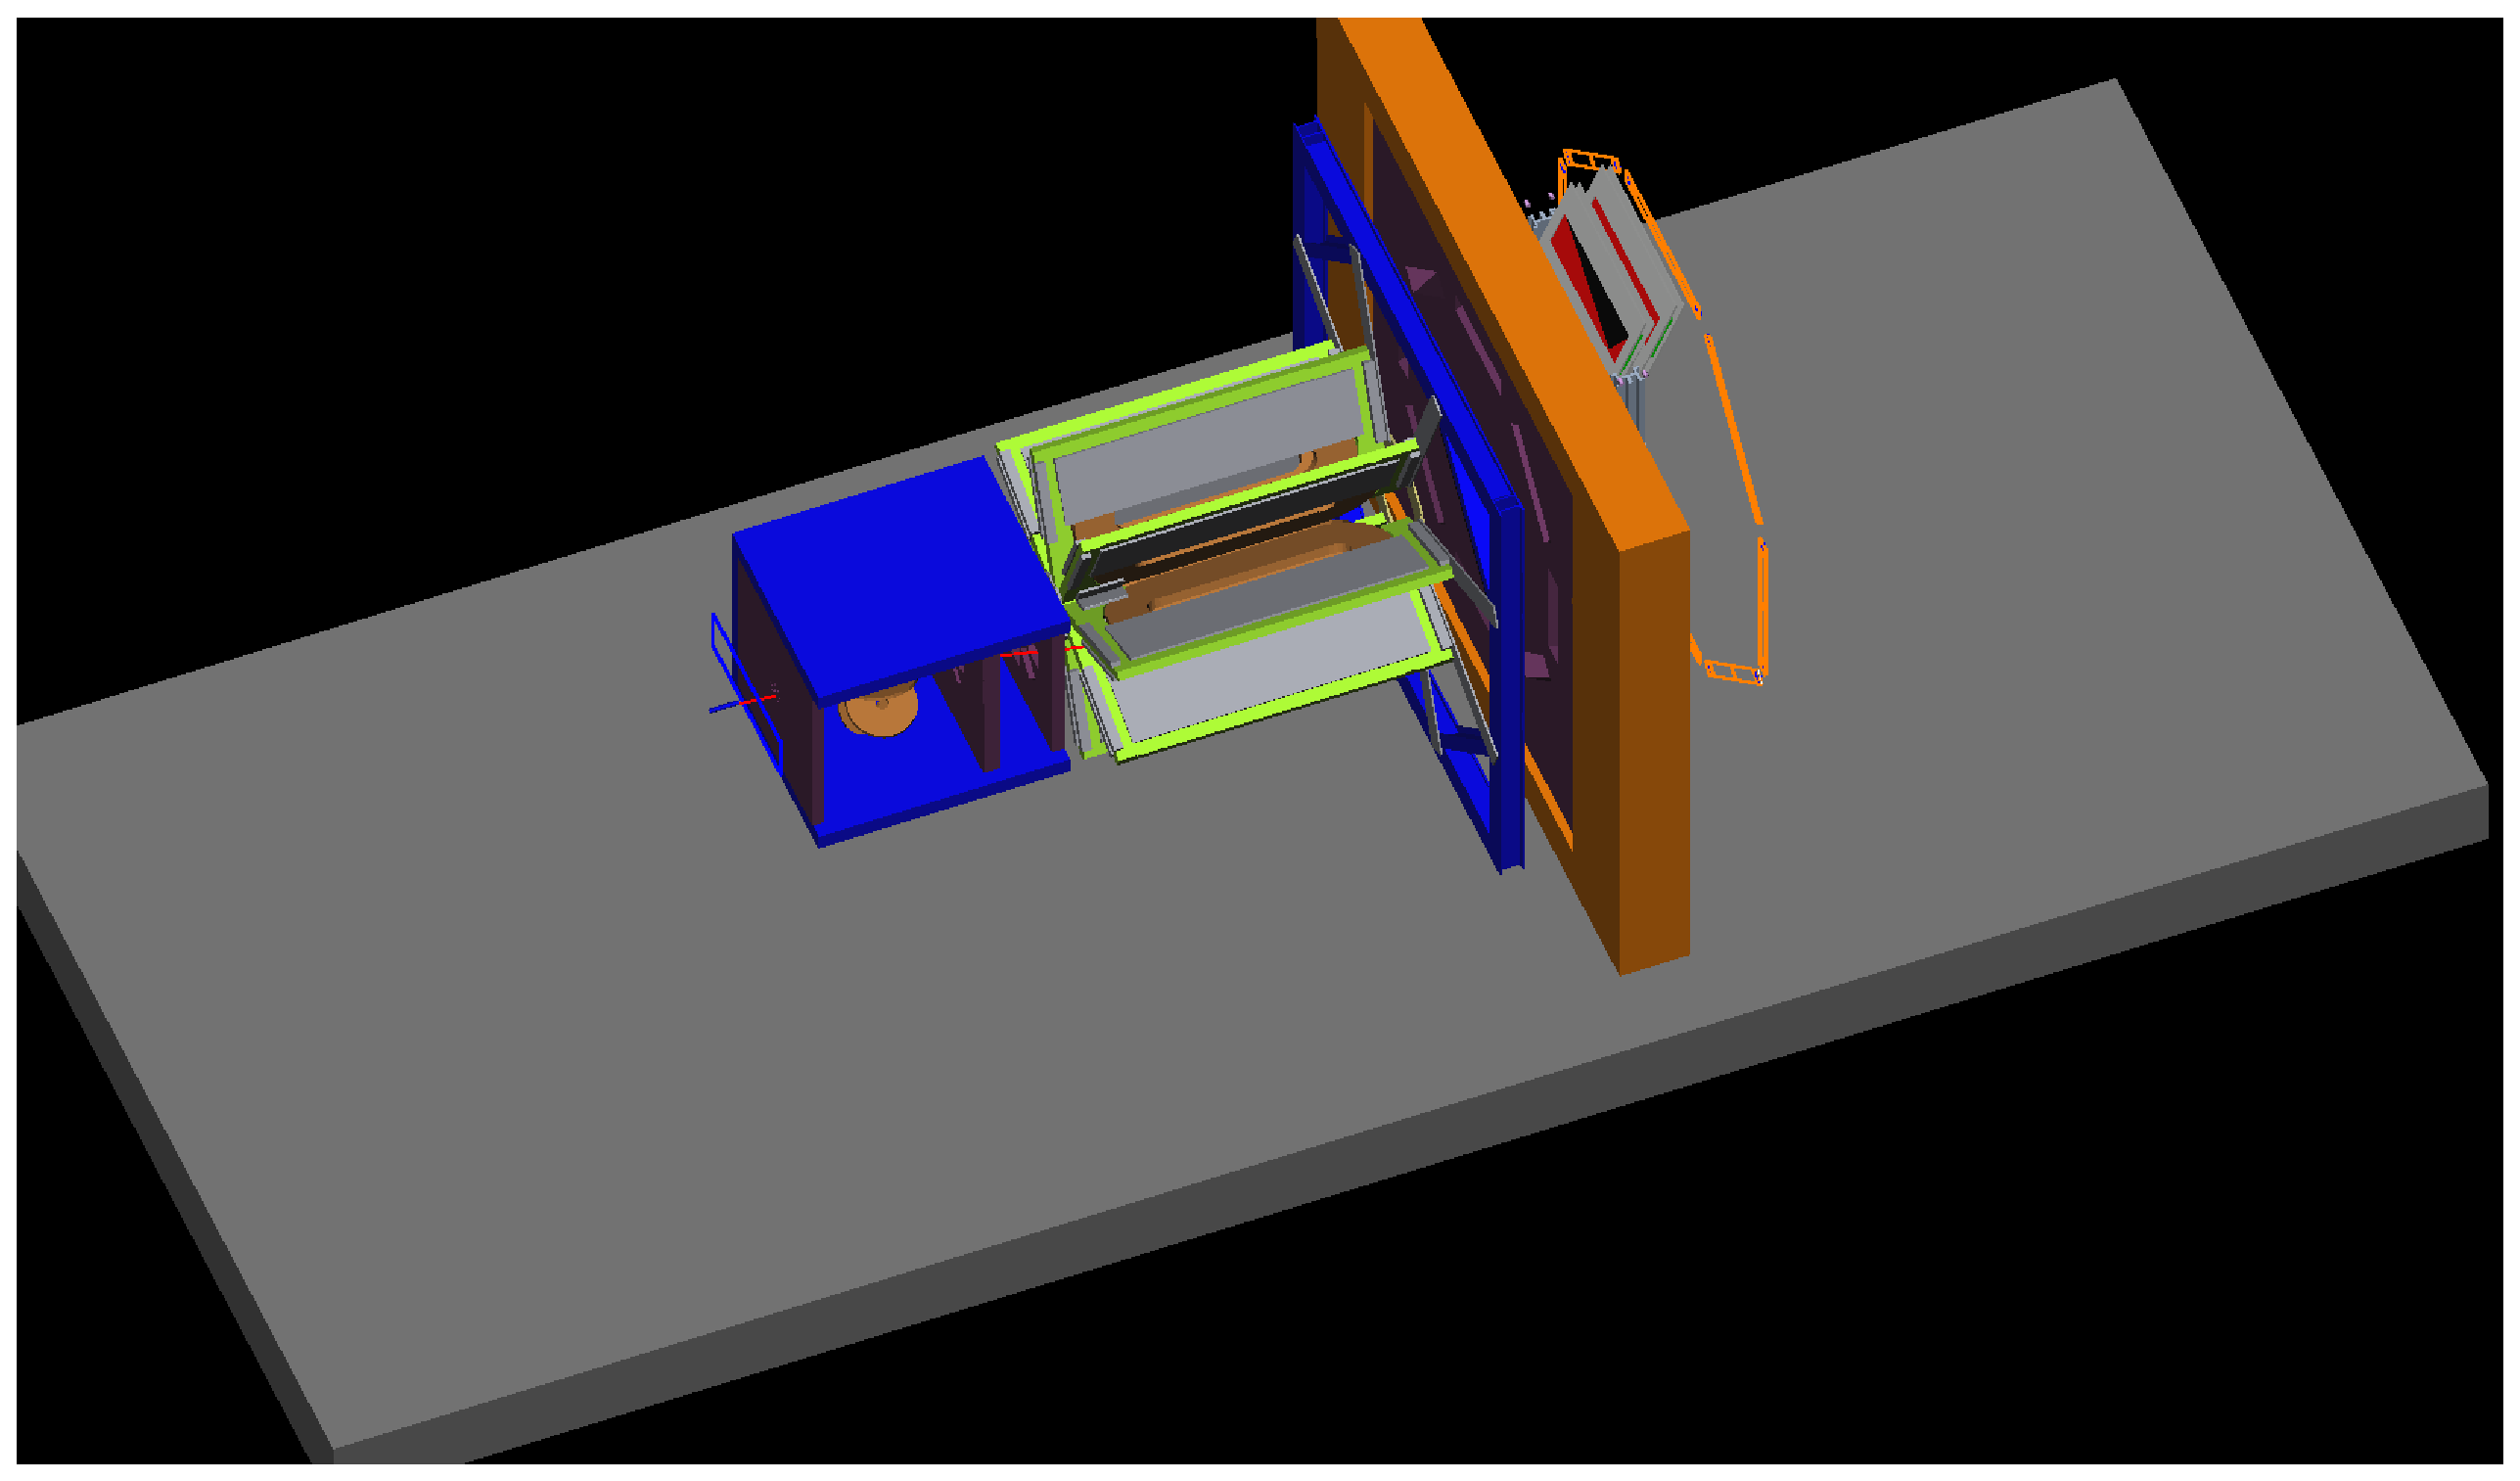
\includegraphics[scale=0.5]{./Introduction/figures/QWeakGeant4.eps}
  \caption{QWeak Geant4 Simulation Setup}
           \label{fig:INTRO-1}
\end{figure}
\end{landscape}

\clearpage

This manual is organized as follows: 

The first chapter consists of very general information, such as a list
of class names and their current status or level of usage in the
simulation, the compile requirements such as the structure of the {\em
Makefile} and where the source files have to be located with respect
to each other, environment variable definitions, etc.. In other words,
this portion of the document should be enough to compile the
simulation as it stands, provided that both ROOT and GEANT4 have been
installed properly. The second chapter provides a detailed description
of the event generator used in the simulations and attempts to give a
detailed explanation of the physics processes included.  The following
chapters (one for each class) provide a detailed reference explaining
what the classes do, how they do it and how to use the routines to
access the class members, change variables, etc.. This portion is
necessary for someone who actually wants to change the code. The
details about the implementation of the physics processes used in the
simulation are given together with its code in the appropriate
chapters.

%{\bf A note with regard to coding conventions: I don't use them.}  I
%never do, unless I am forced to by the syntax of the programming
%language.  What would life be without a little variation :). I have
%put little to no effort into making the code ``look'' pretty nor can I
%claim to have always used names for variables, defines, or constants
%that make sense ( I try to though).  If I had had the time to do that
%I would have gotten a second job as a programmer. So if you want to
%utter complaints regarding those issues, direct them where you are
%supposed to: at your spouse or random people {\bf other than me}.
%One thing I do do, however, is to make sure that my classes are well
%written; the way they are supposed to in the object oriented
%programming paradigm. So you should be able to use them as a black
%box. If you don't know what I mean, you can refer to any basic C++ 
%book.

 
